\documentclass[LPSC_Labo03_SDeriaz]{subfiles}



\begin{document}
\section{Analyse}
\subsection{Virgule fixe}
Comme les calculs sont réalisés sur FPGA, il est plus adapté d'utiliser des nombres en virgule fixe. Étant donné que les DSP sont sur 18 bits, les nombres seront eux aussi sur 18 bits avec :
\begin{itemize}
\item Un bit de signe
\item Deux bits avant la virgule (pour écrire des nombres entre 3 et -4)
\item Quinze bits après la virgule ce qui permet d'avoir une résolution de \num{3.05e-5}
\end{itemize}
\subsection{Organisation}
La base du calcul (l'itérateur) sera réalisé en premier. Il s'agit d'un bloc VHDL capable d'effectuer le calcul
$$z_{k+1}=z_{k}^2+C$$
Tout en indiquant si le rayon limite est atteint et le nombre d'itérations en sortie. Si l'entrée \verb!done_in! est activée, alors le nombre d'itérations en sortie est le même que le nombre d'itérations en entrée.
\begin{figure}[H]
\centering
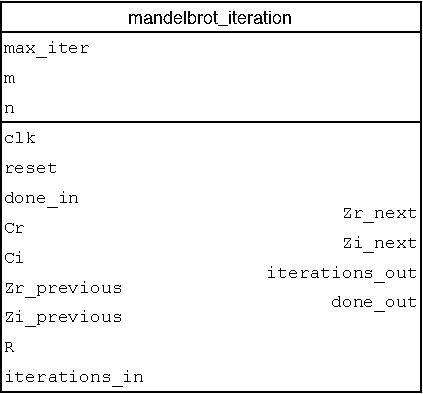
\includegraphics[scale=0.75,page=1]{../Documents/Schemas-crop.pdf}
\caption[caption]{Bloc \texttt{mandelbrot\_iteration}}
\end{figure}
Ce bloc sera ensuite réutilisé dans deux versions du programme
\begin{enumerate}
\item Bouclage sur lui-même (loop) pour calculer un pixel à la fois
\item Pipeline, 100 itérateurs (le nombre maximal d'itérations) sont reliés les uns après les autres ce qui permet de calculer un pixel par coup d'horloge
\end{enumerate}
\subsubsection{Bouclage}
Les sorties de l'itérateur sont reliées sur les entrées à l'exception du premier itérateur (qui prend les entrées pour le point à calculer) et du dernier (qui fourni le nombre d'itérations en sortie)
\begin{figure}[H]
\centering
\includegraphics[scale=0.75,page=2]{../Documents/Schemas-crop.pdf}
\caption[caption]{Bloc \texttt{mandelbrot\_loop}}
\end{figure}
\subsubsection{Pipeline}
Les itérateurs sont reliés à la suite les uns des autres, les entrées \verb!Cr! et \verb!Ci! sont propagées aux même rythme que le pipeline (registres à la suite)
\begin{figure}[H]
\centering
\includegraphics[width=\textwidth,page=3]{../Documents/Schemas-crop.pdf}
\caption[caption]{Bloc \texttt{mandelbrot\_pipeline}}
\end{figure}




\subsection{Calculs sur Python}
Avant d'implémenter la fractale sur FPGA, il est souhaitable d'avoir un modèle complet pour comparer et débugger le système. Le modèle sera réalisé dans Python en utilisant le package \verb!fixedpoint!\footnote{\url{https://pypi.org/project/fixedpoint/}}. De cette façon il est possible d'effectuer les calculs en virgule flottante (pour avoir la "vraie" fractale) puis les mêmes calculs en virgule fixe afin de comparer de pouvoir créer un banc de test VHDL.
\begin{figure}[H]
\centering
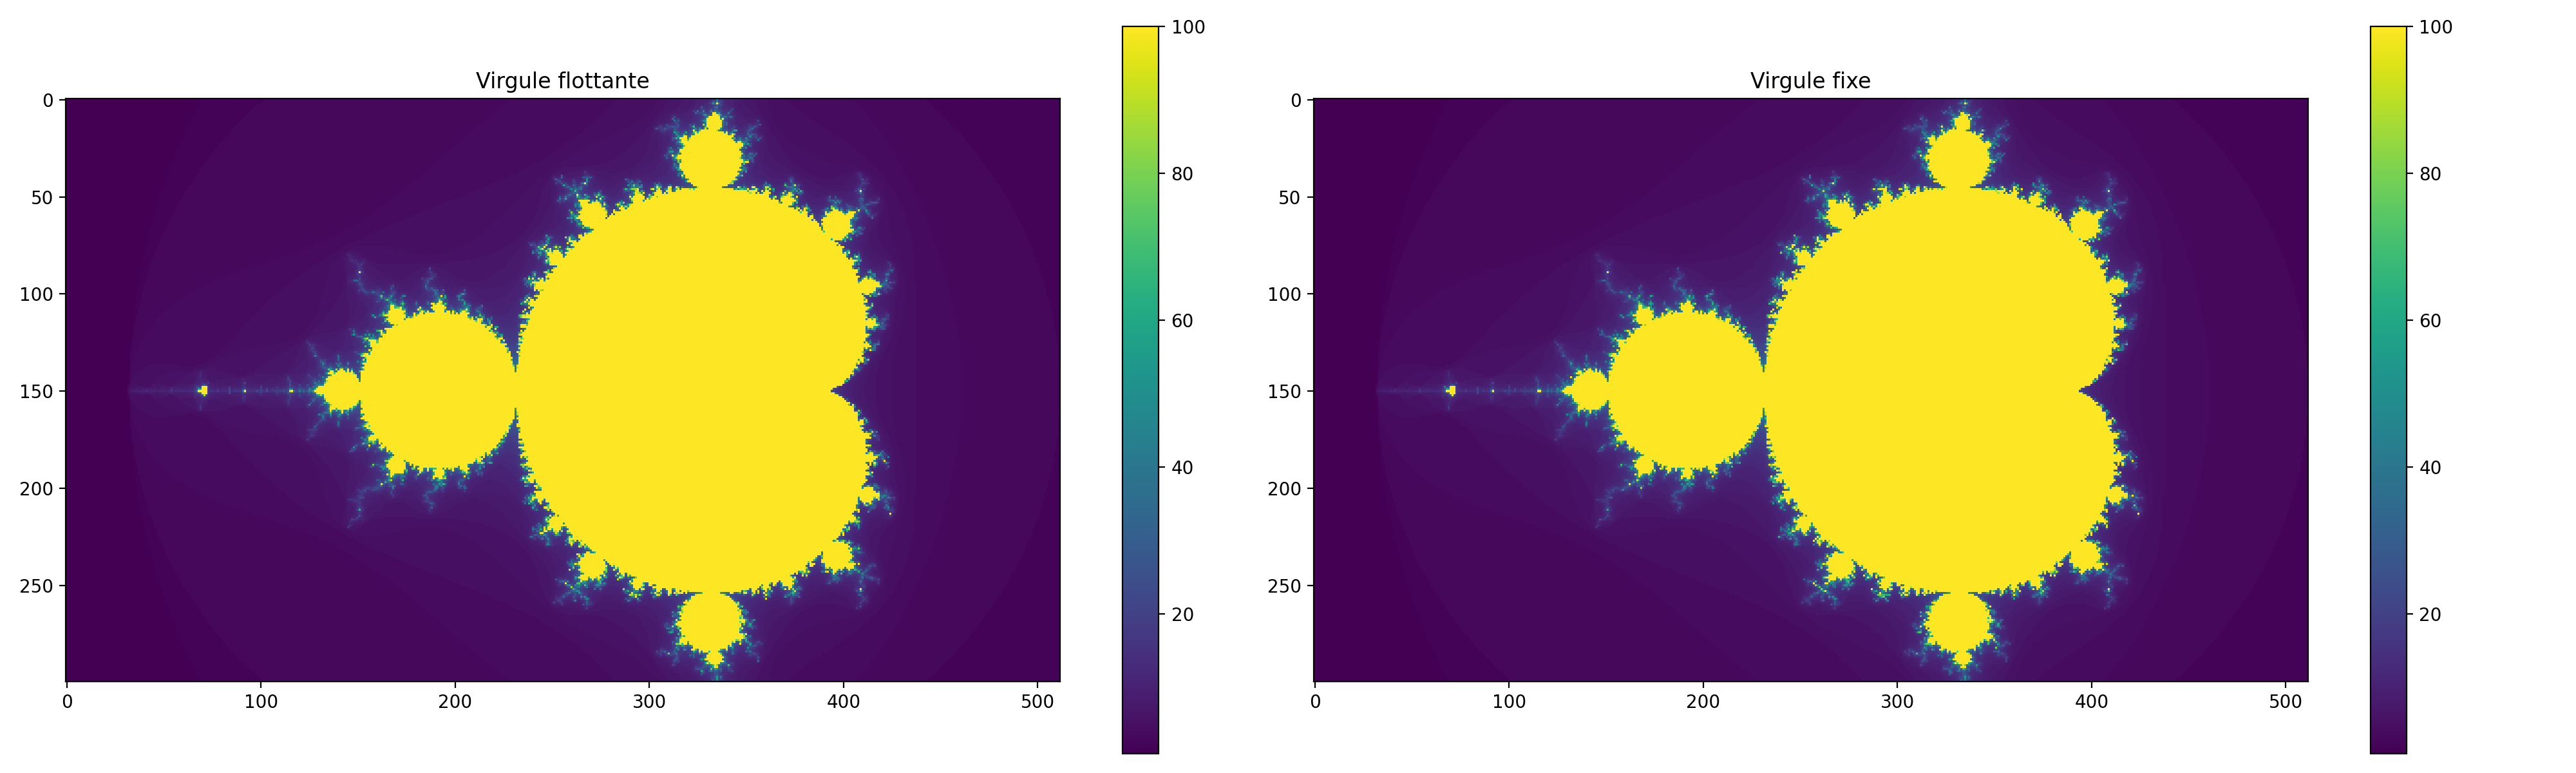
\includegraphics[width=\textwidth]{mandelbrot_comparaison.png}
\caption{Fractales avec virgule fixe et virgule flottante}
\end{figure}
\begin{figure}[H]
\centering
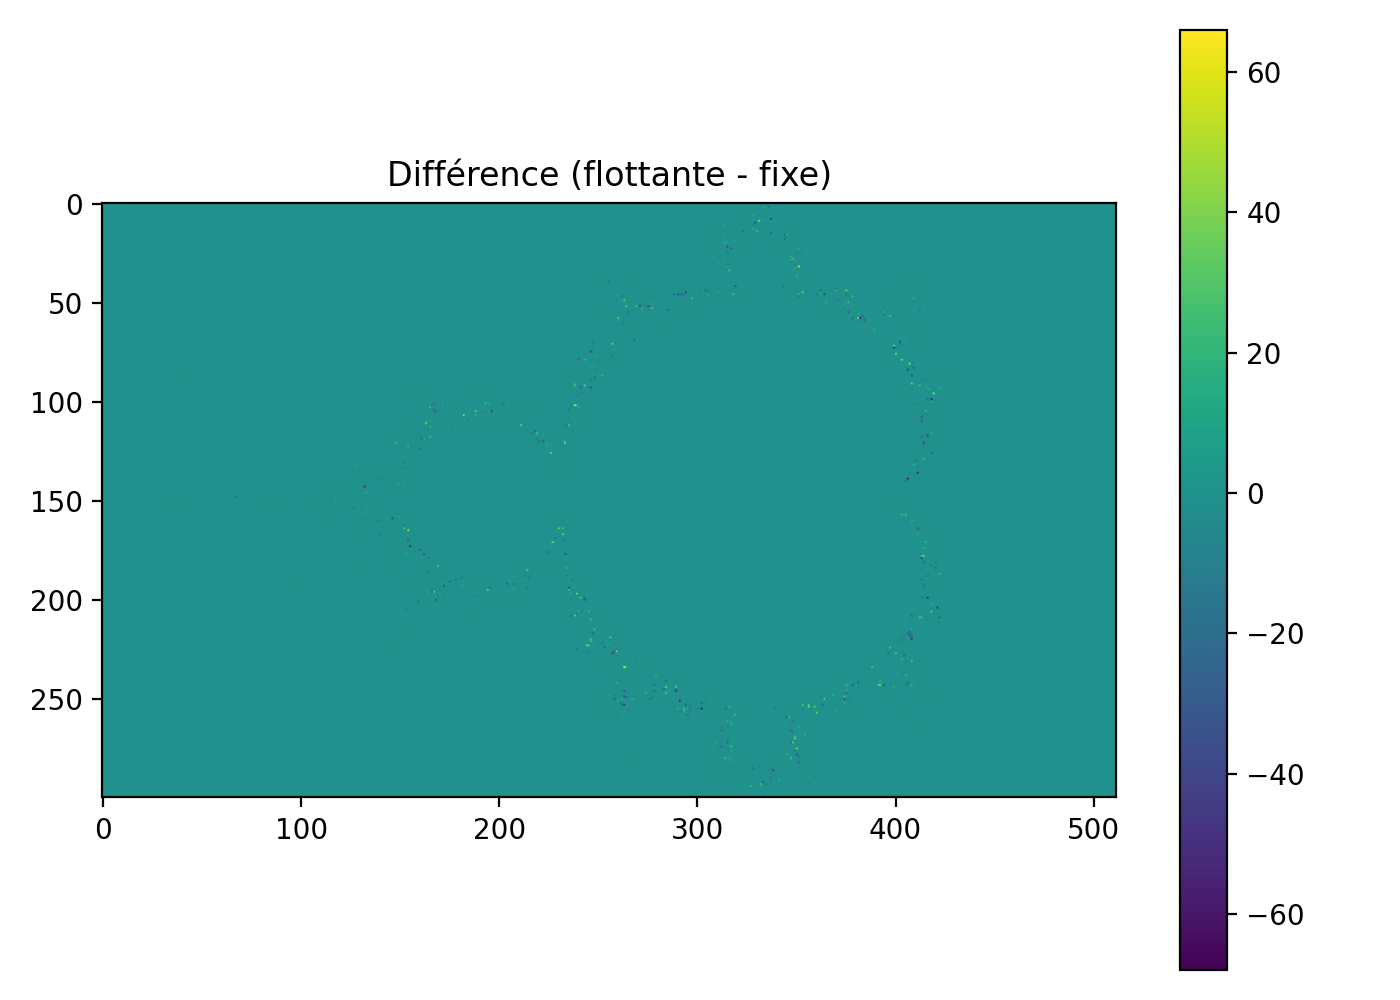
\includegraphics[scale=0.4]{mandelbrot_difference.png}
\caption{Différence entre les deux résultats}
\end{figure}
On remarque qu'il existe une différence entre les deux approches (à cause des arrondis), notamment sur les bords de la figure centrale, mais elle est négligeable dans notre application car elle n'impacte pas le rendu visuel.





\subsection{Couleurs}
Afin de déterminer les couleurs de chaque pixel en fonction du nombre d'itérations, on utilise une interpolation sur des points donnés pour chaque couleur (rouge, vert, bleu). Il existe plusieurs choix, mais le celui donné par cette réponse\footnote{\url{https://stackoverflow.com/a/25816111/8418125}} donne un bon résultat
\begin{figure}[H]
\centering
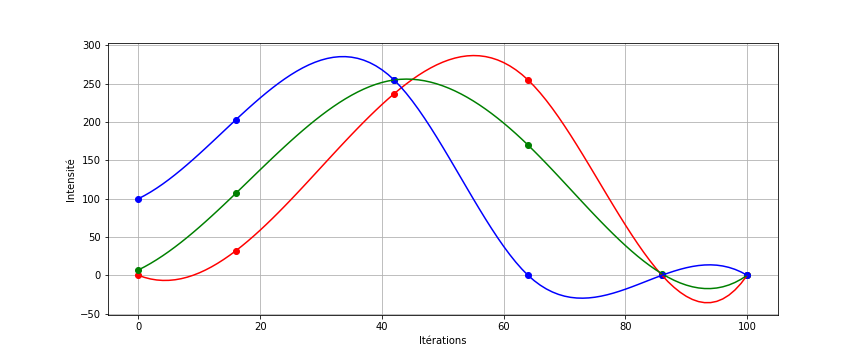
\includegraphics[width=12cm]{LUT_points.png}
\caption{Interpolation cubique sur les couleurs}
\end{figure}
Après ajustage (pour borner les intensités entre 0 et 255), on obtient la répartition de couleurs suivante en fonction du nombre d'itérations :
\begin{figure}[H]
\centering
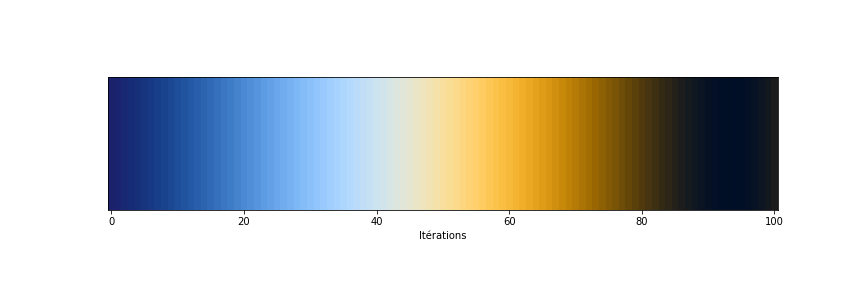
\includegraphics[width=12cm]{LUT.png}
\caption{LUT pour la couleur de chaque pixel en fonction des itérations}
\end{figure}
La LUT est auto-générée dans un package VHDL.

\end{document}